\section{Tests de validations et fonctionnement}

\subsection{Test unitaires}

Afin de vérifier la validité de chacune des fonctions écrites, nous avons comparé les resultats des versions Lua et Java. Les exceptions Lua et Java ne sont pas converties par l'autre langage. Ainsi lorsque le programme rencontre une erreur dans la partie java ou la partie Lua, il ne retourne aucune exception. Nous avons donc dû effectuer de nombreux affichages dans les différentes fonctions pour pouvoir suivre l'execution du programme et savoir quelles fonctions provoquait l'erreur. 

\subsection{Test globaux}

La complexité de Prestaf peut atteindre $O(2^{2^{2^{pn}}})$ pour les quantificateurs. Il est donc très difficile de tester des grandes formules. De plus, le nombre d'état peut facilement devenir très important comme présenté dans la figure \ref{image1}. Les graphes générés deviennent alors illisibles.\par

Nous avons donc choisi d'effectuer la pluspart de nos tests de l'application sur des formules contenant peu de variables, afin de pouvoir comparer les graphes obtenus par la nouvelle version de Presburger et l'ancienne. Nous avons également effectuer quelques tests sur de grandes formules, pour vérifier si l'application affichait un graphe.\clearpage

\begin{figure}[h]

\centering

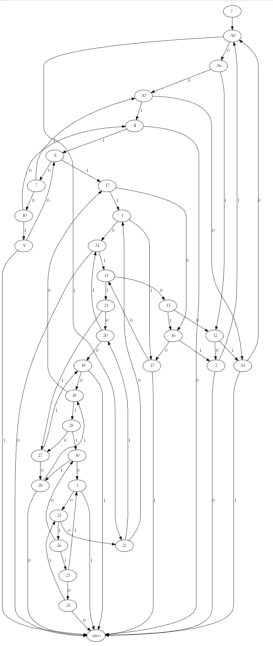
\includegraphics[scale=0.5]{graphe.png}

\caption{Graphe généré pour $3w+x-y=z$}
\label{image1}
\end{figure}
